\documentclass[aspectratio=169]{../latex_main/tntbeamer}  % you can pass all options of the beamer class, e.g., 'handout' or 'aspectratio=43'
\usepackage{dsfont}
\usepackage{bm}
\usepackage[english]{babel}
\usepackage[T1]{fontenc}
%\usepackage[utf8]{inputenc}
\usepackage{graphicx}
\graphicspath{ {./figures/} }
\usepackage{algorithm}
\usepackage[ruled,vlined,algo2e,linesnumbered]{algorithm2e}
\usepackage{hyperref}
\usepackage{booktabs}
\usepackage{mathtools}

\usepackage{amsmath,amssymb}

\DeclareMathOperator*{\argmax}{arg\,max}
\DeclareMathOperator*{\argmin}{arg\,min}

\usepackage{amsbsy}
\newcommand{\vect}[1]{\bm{#1}}
%\newcommand{\vect}[1]{\boldsymbol{#1}}

\usepackage{pgfplots}
\pgfplotsset{compat=1.16}
\usepackage{tikz}
\usetikzlibrary{trees} 
\usetikzlibrary{shapes.geometric}
\usetikzlibrary{positioning,shapes,shadows,arrows,calc,mindmap}
\usetikzlibrary{positioning,fadings,through}
\usetikzlibrary{decorations.pathreplacing}
\usetikzlibrary{intersections}
\pgfdeclarelayer{background}
\pgfdeclarelayer{foreground}
\pgfsetlayers{background,main,foreground}
\tikzstyle{activity}=[rectangle, draw=black, rounded corners, text centered, text width=8em]
\tikzstyle{data}=[rectangle, draw=black, text centered, text width=8em]
\tikzstyle{myarrow}=[->, thick, draw=black]

% Define the layers to draw the diagram
\pgfdeclarelayer{background}
\pgfdeclarelayer{foreground}
\pgfsetlayers{background,main,foreground}

% Requires XeLaTeX or LuaLaTeX
%\usepackage{unicode-math}

\usepackage{fontspec}
%\setsansfont{Arial}
\setsansfont{RotisSansSerifStd}[ 
Path=../latex_main/fonts/,
Extension = .otf,
UprightFont = *-Regular,  % or *-Light
BoldFont = *-ExtraBold,  % or *-Bold
ItalicFont = *-Italic
]
\setmonofont{Cascadia Mono}[
Scale=0.8
]

% scale factor adapted; mathrm font added (Benjamin Spitschan @TNT, 2021-06-01)
%\setmathfont[Scale=1.05]{Libertinus Math}
%\setmathrm[Scale=1.05]{Libertinus Math}

% other available math fonts are (not exhaustive)
% Latin Modern Math
% XITS Math
% Libertinus Math
% Asana Math
% Fira Math
% TeX Gyre Pagella Math
% TeX Gyre Bonum Math
% TeX Gyre Schola Math
% TeX Gyre Termes Math

% Literature References
\newcommand{\lit}[2]{\href{#2}{\footnotesize\color{black!60}[#1]}}

%%% Beamer Customization
%----------------------------------------------------------------------
% (Don't) Show sections in frame header. Options: 'sections', 'sections light', empty
\setbeamertemplate{headline}{empty}

% Add header logo for normal frames
\setheaderimage{
	% 
\includegraphics[height=\logoheight]{figures/TNT_darkv4.pdf}
	
\includegraphics[height=\logoheight]{../latex_main/figures/luh_logo_rgb_0_80_155.pdf}
	% 
\includegraphics[height=\logoheight]{figures/logo_tntluh.pdf}
}

% Header logo for title page
\settitleheaderimage{
	% 
\includegraphics[height=\logoheight]{figures/TNT_darkv4.pdf}
	
\includegraphics[height=\logoheight]{../latex_main/figures/luh_logo_rgb_0_80_155.pdf}
	% 
\includegraphics[height=\logoheight]{figures/logo_tntluh.pdf}
}

% Title page: tntdefault 
\setbeamertemplate{title page}[tntdefault]  % or luhstyle
% Add optional title image here
%\addtitlepageimagedefault{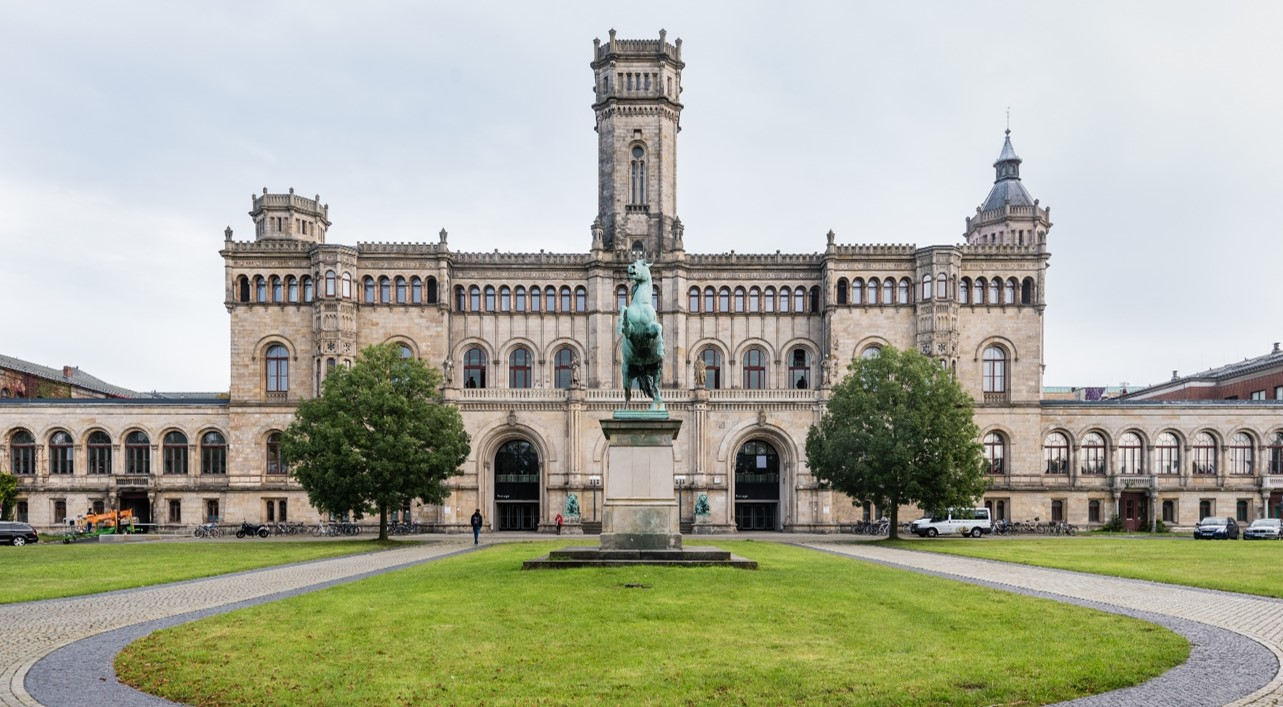
\includegraphics[width=0.65\textwidth]{figures/luh_default_presentation_title_image.jpg}}

% Title page: luhstyle
% \setbeamertemplate{title page}[luhstyle]
% % Add optional title image here
% \addtitlepageimage{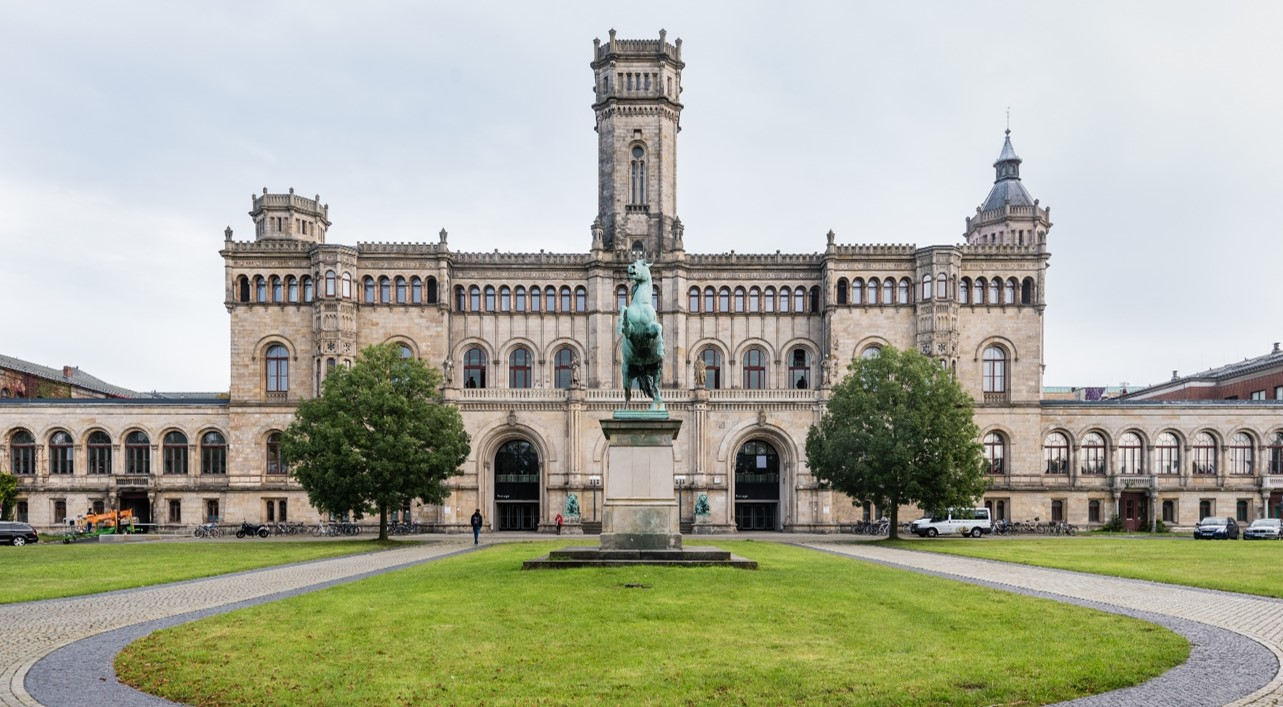
\includegraphics[width=0.75\textwidth]{figures/luh_default_presentation_title_image.jpg}}

\author[Abedjan \& Lindauer]{Ziawasch Abedjan \& Marius Lindauer\\[1em]
	
\includegraphics[height=\logoheight]{../latex_main/figures/luh_logo_rgb_0_80_155.pdf}\qquad
	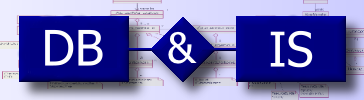
\includegraphics[height=\logoheight]{../latex_main/figures/DBIS_Kurzlogo.png}\qquad

\includegraphics[height=\logoheight]{../latex_main/figures/TNT_darkv4}\qquad

\includegraphics[height=\logoheight]{../latex_main/figures/L3S.jpg}	}
\date{Summer Term 2022; \hspace{0.5em} {
\includegraphics[height=1.5em]{../latex_main/figures/Cc-by-nc-sa_icon.svg.png}}; based on \href{https://ds100.org/fa21/}{[DS100]}
}


%%% Custom Packages
%----------------------------------------------------------------------
% Create dummy content
\usepackage{blindtext}

% Adds a frame with the current page layout. Just call \layout inside of a frame.
\usepackage{layout}


%%% Macros
%\renewcommand{\vec}[1]{\mathbf{#1}}
% \usepackage{bm}
%\let\vecb\bm

\title[Introduction]{DS: Regular Expressions}
\subtitle{Regular Expression Basics}

\graphicspath{ {./figure/} }
%\institute{}


\begin{document}
	
	\maketitle
	\begin{frame}{Extracting Date Information}
	    Earlier we saw that we can hack together code that uses split to extract info:\\
	    \begin{figure}
	        \centering
	        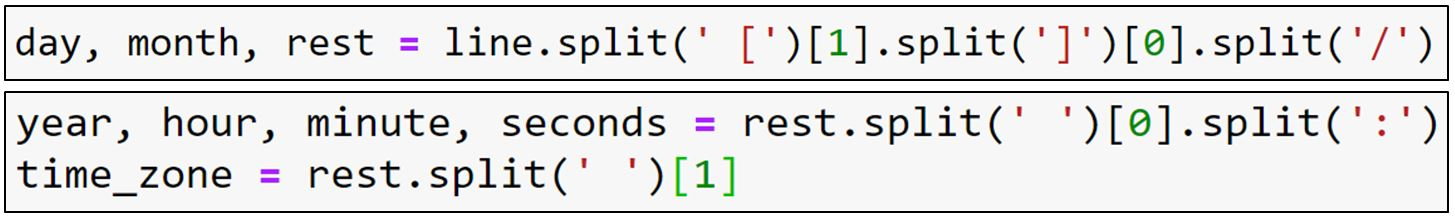
\includegraphics[scale=.35]{Bild6}
	    \end{figure}
	    An alternate approach is to use a so-called “regular expression”:
        \begin{itemize}
            \item Implementation provided in the re library built into Python
            \item We’ll spend some time today working up to expressions like shown 
        \end{itemize}
        \begin{figure}
	        \centering
	        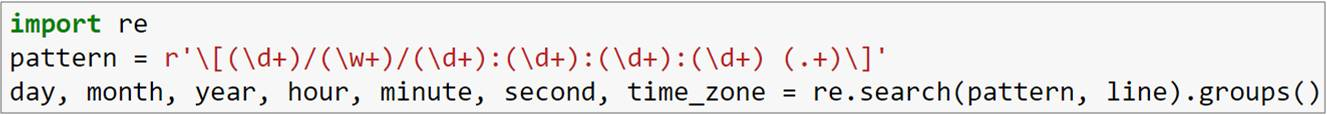
\includegraphics[scale=.6]{Bild7}
	    \end{figure}
	\end{frame}
	
	
	
	
	\begin{frame}{Regular Expressions}
	    A formal language is a set of strings, typically described implicitly.
	    \begin{itemize}
	        \item Example: “The set of all strings of length < 10 that contain ‘horse’”
	    \end{itemize}
	    A regular language is a formal language that can be described by a regular expression (which we will define soon). 
        \begin{figure}
	        \centering
	        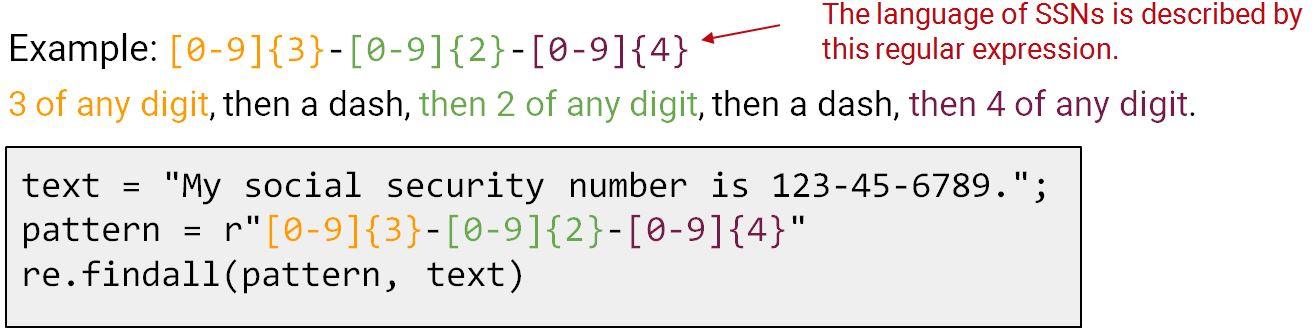
\includegraphics[scale=.44]{Bild8}
	    \end{figure}
	\end{frame}
	
	
	
	\begin{frame}{\url{Regex101.com} (or the online tutorial \url{regexone.com})}
	    There are a ton of nice resources out there to experiment with regular expressions (e.g. \url{Regex101.com}, \url{regexone.com}, sublime text, python, etc).\\
	    I recommend trying out \url{Regex101.com}, which provides a visually appealing and easy to use platform for experimenting with regular expressions.
        \begin{itemize}
            \item Example: \url{https://regex101.com/r/1SREie/1}
        \end{itemize}
        \begin{figure}
	        \centering
	        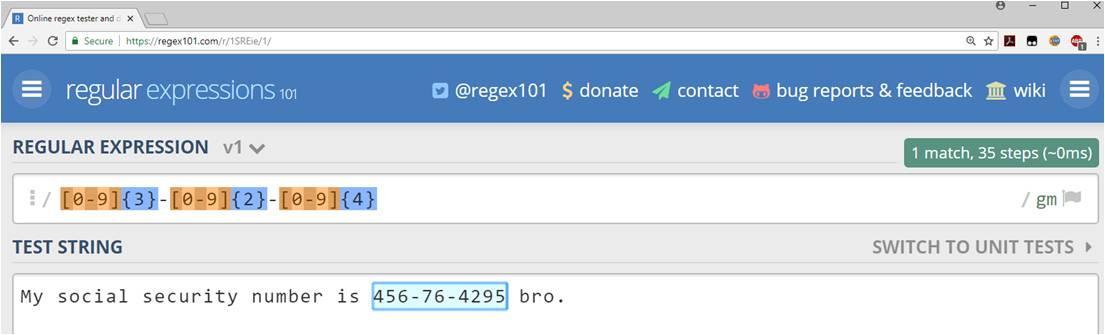
\includegraphics[scale=.6]{Bild9}
	    \end{figure}
	\end{frame}
	
	
	
	\begin{frame}{Regular Expression Syntax}
	   The four basic operations for regular expressions.
        \begin{itemize}
            \item Can technically do anything with just these basic four (albeit tediously). 
        \end{itemize}
        \begin{figure}
	        \centering
	        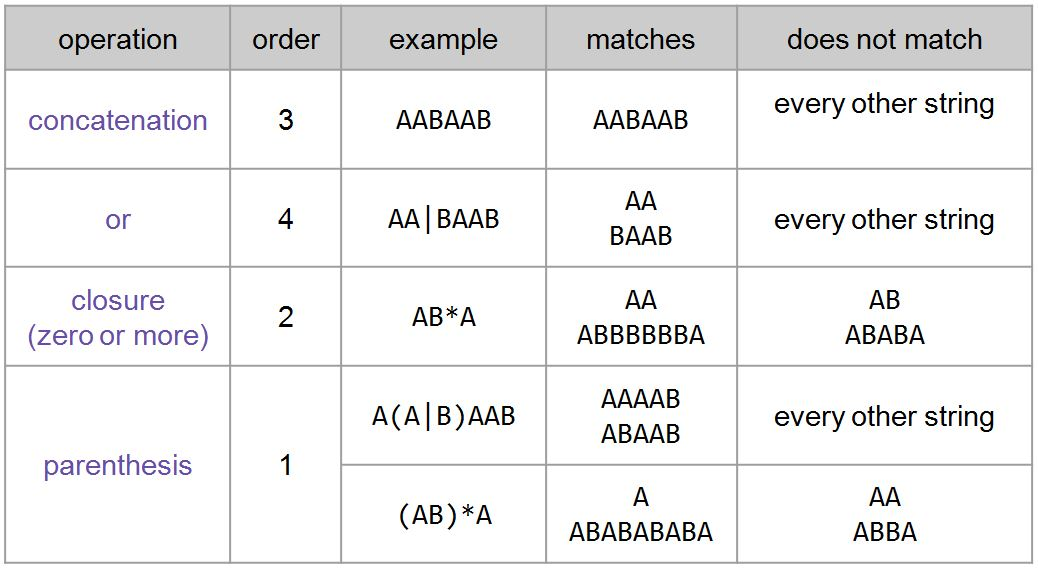
\includegraphics[scale=.35]{Bild10}
	    \end{figure}
	\end{frame}
	
	
	
	\begin{frame}{Regular Expression Syntax}
	   AB*: A then zero or more copies of B: A, AB, ABB, ABBB\\
       (AB)*: Zero or more copies of AB: ABABABAB,  ABAB, AB,  

        \begin{figure}
	        \centering
	        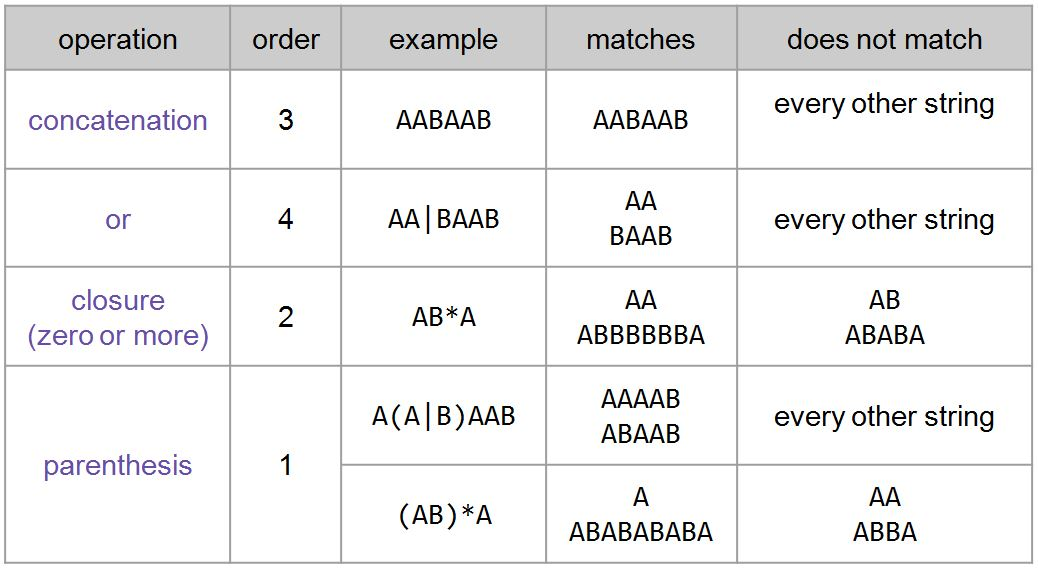
\includegraphics[scale=.35]{Bild10}
	    \end{figure}
	\end{frame}
	
	
	
	\begin{frame}{Puzzle: Use regex101.com to test! Or \url{tinyurl.com/reg913z}}
 

        \begin{figure}
	        \centering
	        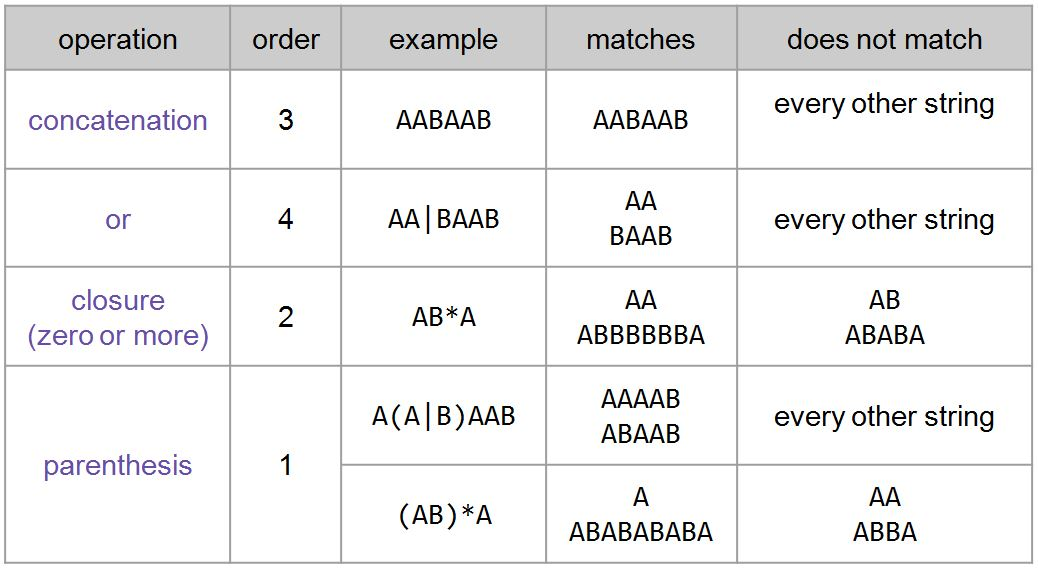
\includegraphics[scale=.35]{Bild10}
	    \end{figure}
	    Give a regular expression that matches moon, moooon, etc. Your expression should match any even number of os except zero (i.e. don’t match mn).

	\end{frame}
	
	
	\begin{frame}{Puzzle Solution}
 

        \begin{figure}
	        \centering
	        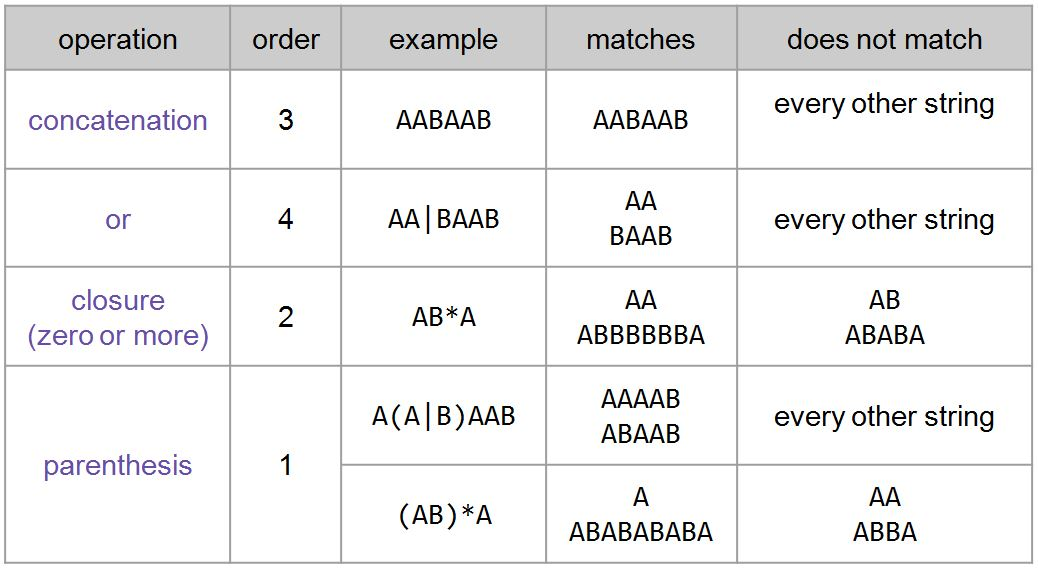
\includegraphics[scale=.35]{Bild10}
	    \end{figure}
	    Solution to puzzle on previous slide: moo(oo)*n

	\end{frame}
	
	
	
	\begin{frame}{Regular Expression moo(oo)*n: \url{https://tinyurl.com/reg913m}}
 

        \begin{figure}
	        \centering
	        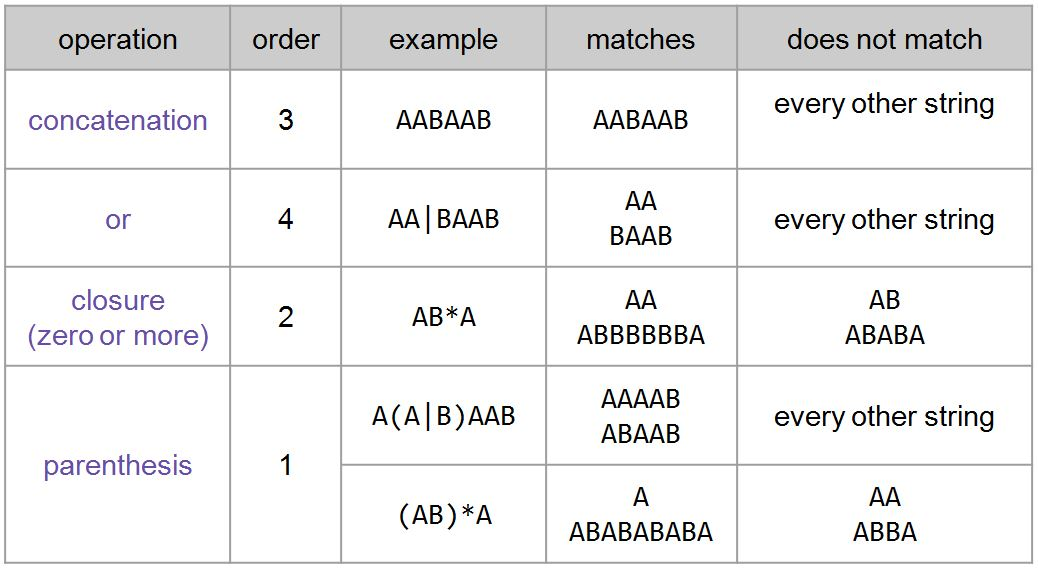
\includegraphics[scale=.35]{Bild10}
	    \end{figure}
	    Give a regex that matches muun, muuuun, moon, moooon, etc. Your expression should match any even number of us or os except zero (i.e. don’t match mn).


	\end{frame}
	
	
	
	\begin{frame}{Puzzle Solution}
 

        \begin{figure}
	        \centering
	        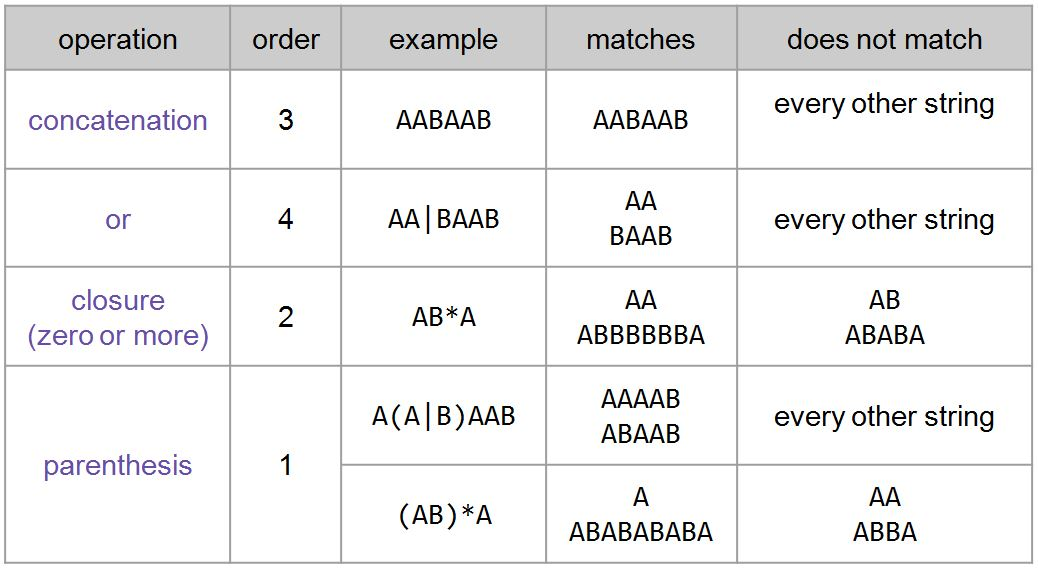
\includegraphics[scale=.35]{Bild10}
	    \end{figure}
	    Solution to puzzle on previous slide: m(uu(uu)*|oo(oo)*)n
        \begin{itemize}
            \item Note: m(uu(uu)*)|(oo(oo)*)n is not correct! OR must be in parentheses!
        \end{itemize}

	\end{frame}
	
	
	
	\begin{frame}{Order of Operations in Regexes}
 
        m(uu(uu)*|oo(oo)*)n
        \begin{itemize}
            \item Matches starting with m and ending with n, with either of the following in the middle:
            \begin{itemize}
                \item uu(uu)* \hspace{3cm} Match examples: muun, muuuun
                \item oo(oo)*  \hspace{3cm} Match examples: moon, moooon  
            \end{itemize}
        \end{itemize}
        \pause
        m(uu(uu)*)|(oo(oo)*)n\\
        \bigskip
        \begin{itemize}
            \item Matches either of the following
            \begin{itemize}
                \item m followed by uu(uu)*  \hspace{3cm} Match examples: muu, muuuu
                \item oo(oo)* followed by n  \hspace{3cm} Match examples: oon, oooon  
            \end{itemize}
        \end{itemize}
        \bigskip
        In regexes | comes last.

	\end{frame}
\end{document}